\subsection{Przeprowadzić uczenie ostatniej warstwy splotowej wraz z częścią
klasyfikującą}

Ostatnią warstwą splotową w sieci EfficientNetB0 jest warstwa top\_conv, która jest trzecią warstwą od góry. Z tego powodu zamrożono wszystkie warstwy sieci poza trzema ostatnimi. Jako wagi początkowe zastosowano wagi imagenet. Następnie przeprowadzono uczenie z wykorzystaniem zbioru treningowego. W trakcie uczenia zastosowano optymalizator Adam, funkcję straty sparse categorical crossentropy oraz metrykę accuracy. Przetestowano różne wartości współczynnika uczenia, ostatecznie wybrano wartość 1e-5. Po 40 epokach uczenia osiągnięto na zbiorze testowym \textbf{accuracy na poziomie 0.74, loss na poziomie 0.66} oraz macierz pomyłek przedstawioną w tabeli \ref{tab:z2a}. Wyniki uczenia w czasie przedstawiono na rysunku \ref{fig:z2a}. Dalsze uczenie nie przynosiło poprawy wyników.

% Confusion Matrix:
%  [[ 32  18  29  49]
%  [  0 229   4   1]
%  [  1   4 105   1]
%  [  4  19  24  76]]

\begin{table}[H]
\centering
\begin{tabular}{|c|c|c|c|c|}
\hline
klasa & 0 & 1 & 2 & 3 \\ \hline
0 & 32 & 18 & 29 & 49 \\ \hline
1 & 0 & 229 & 4 & 1 \\ \hline
2 & 1 & 4 & 105 & 1 \\ \hline
3 & 4 & 19 & 24 & 76 \\ \hline
\end{tabular}
\caption{Macierz pomyłek dla zadania 2a}
\label{tab:z2a}
\end{table}

\begin{figure}[H]
    \centering
    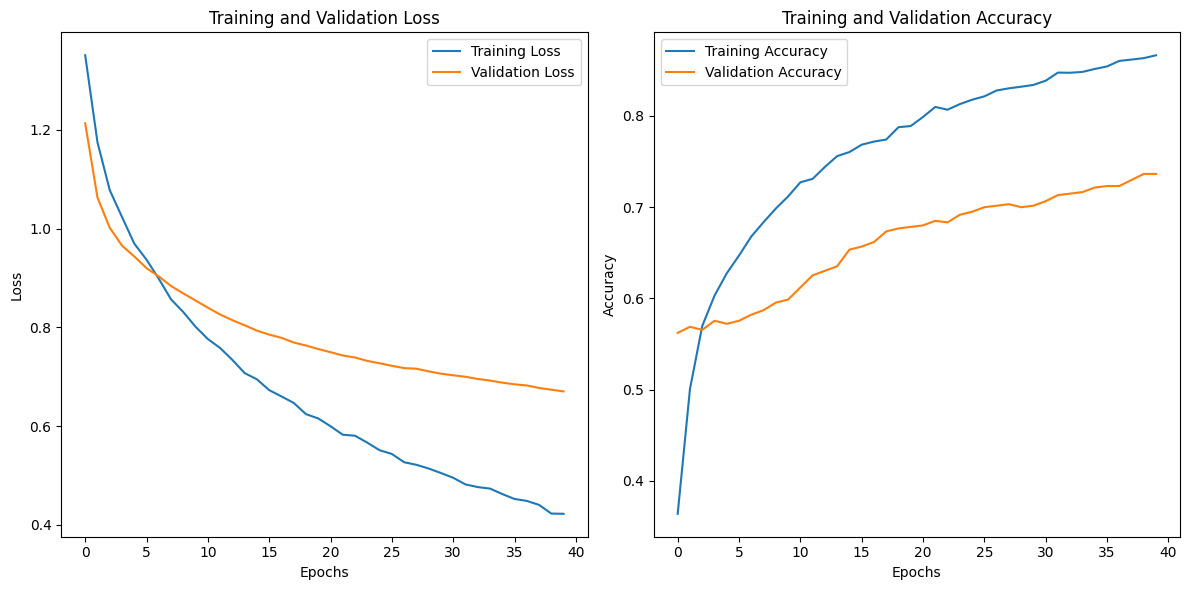
\includegraphics[width=0.8\textwidth]{img/z2a.png}
    \caption{Wyniki uczenia dla zadania 2a}
    \label{fig:z2a}
\end{figure}




%ile parametrów trainable

\subsection{Wytrenować całą sieć dla zadanych danych}
W tym zadaniu odmrożono wszystkie warstwy EfficientNetB0 i nadano im wagi początkowe imagenet. Następnie przeprowadzono uczenie z wykorzystaniem zbioru treningowego. W trakcie uczenia zastosowano optymalizator Adam, funkcję straty sparse categorical crossentropy oraz metrykę accuracy. Przetestowano różne wartości współczynnika uczenia, ostatecznie wybrano wartość 1e-5. Podczas uczenia zastosowano mechanizm early stopping, który zatrzymywał uczenie jeśli przez 4 epoki nie następowała poprawa wyników. Uczenie zatrzymało się po 22 epokach. Ostatecznie osiągnięto na zbiorze testowym \textbf{accuracy na poziomie 0.63, loss na poziomie 1.01} oraz macierz pomyłek przedstawioną w tabeli \ref{tab:z2b}. Wyniki uczenia w czasie przedstawiono na rysunku \ref{fig:z2b_with_w}.

% Test loss: 1.0159192085266113, Test accuracy: 0.6325503587722778
% Confusion Matrix:
%  [[ 56  17  55   0]
%  [  0 234   0   0]
%  [ 22   1  87   1]
%  [  9  36  78   0]]

\begin{table}[H]
\centering
\begin{tabular}{|c|c|c|c|c|}
\hline
klasa  & 0 & 1 & 2 & 3 \\ \hline
0 & 56 & 17 & 55 & 0 \\ \hline
1 & 0 & 234 & 0 & 0 \\ \hline
2 & 22 & 1 & 87 & 1 \\ \hline
3 & 9 & 36 & 78 & 0 \\ \hline
\end{tabular}
\caption{Macierz pomyłek dla zadania 2b z wagami imagenet}
\label{tab:z2b}
\end{table}
    
\begin{figure}[H]
    \centering
    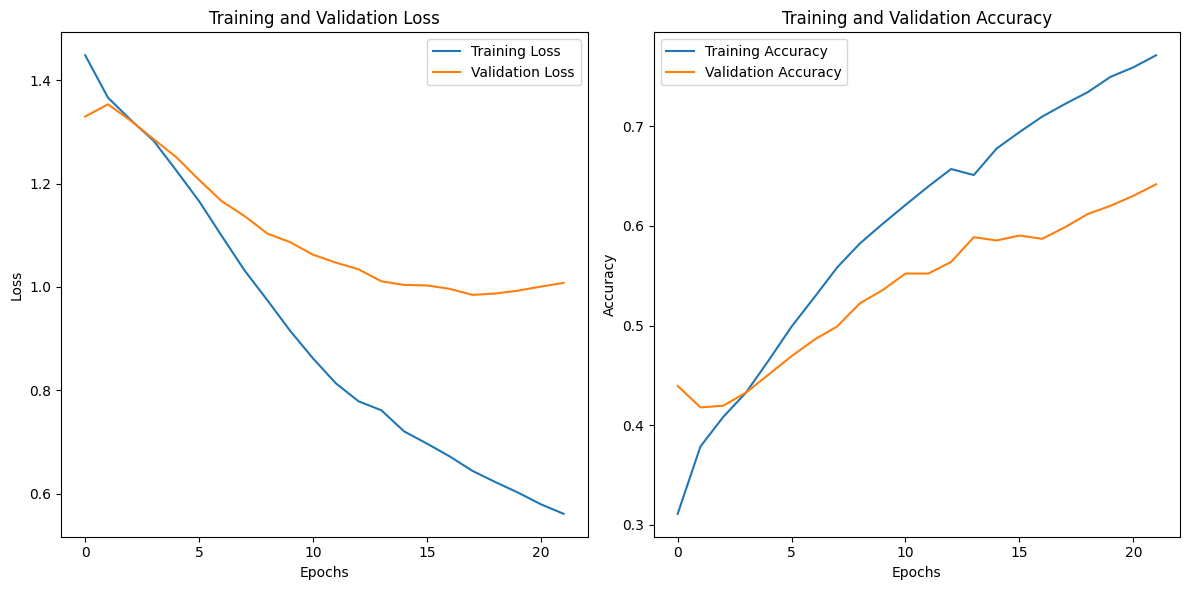
\includegraphics[width=0.8\textwidth]{img/z2b_with_w.png}
    \caption{Wyniki uczenia dla zadania 2b z wagami imagenet}
    \label{fig:z2b_with_w}
\end{figure}

Próbowano także wytrenować całą sieć bez zadanych wag początkowych, jednak w tym przypadku wyniki były dużo gorsze (accuracy na poziomie 0.38). Może to wynikać z faktu, że zbiór treningowy jest stosunkowo mały, a wagi początkowe z imagenet są lepsze niż losowe.

\subsection{Uprościć strukturę sieci wytrenowanej w zadaniu 2c (np. poprzez
usunięcie jednej lub więcej końcowych warstw splotowych, usunięcie
warstw regularyzujących itp.) i ponowić uczenie}

\subsection{Zanalizować wyniki 2 abc}